%xelatex -shell-escape -output-directory=bin ergasia.tex
\documentclass{assignment}

\usepackage{enumerate} % Για την χρησιμοποίηση roman enumerate
\usepackage{pdflscape}

%\university{Πανεπιστήμιο Πειραιώς}{Πα.Πει.}
%\school{Τμήμα Πληροφορικής}{Π.Μ.Σ. "Πληροφορική"}
%\department{Πρόγραμμα Μεταπτυχιακών Σπουδών «Πληροφορική»}{}
%\cover{images/cover.jpg}{http://www.cyberciti.biz/faq/grub-boot-into-single-user-mode/}

\title{Βάσεις Δεδομένων \\ Εργασία Εξαμήνου}
%\projectlevel{Εργαστήριο Λειτουργικά Συστήματα}
%\lesson{Λειτουργικά Συστήματα}{1}
\date{Αθήνα, 2014}

\author{Αναγνωστόπουλος Βασίλης - Θάνος \\ Κατσής Γιώργος}
%\register{ΜΠΠΛ13002}{1}

%\exercauthor{Αναγνωστόπουλος Βασίλης - Θάνος}{06107083}{9}

%\advisor{Τσακίρη Μαρία, Αναπληρώτρια Καθηγήτρια Ε.Μ.Π.}

\begin{document}

\maketitle
% Να σκεφτώ τί αλλαγές θέλω να κάνω με τις αριθμήσεις και άμα θέλω να κάνω.
% Να σκεφτώ να τις ενσωματώσω και στο assignment.cls

\setcounter{page}{1} 
\pagenumbering{roman}

\pagestyle{plain}
\tableofcontents
\listoftables
\listoffigures
\newpage


%\pagestyle{headings}
%\pagestyle{fancy}
\setcounter{page}{1} 
\pagenumbering{arabic}

\section{Εισαγωγή - Αντικείμενο της άσκησης}

Σκοπός της άσκησης είναι η σχεδίαση και υλοποίηση μιας βάσης δεδομένων,
ακολουθώντας τη μεθοδολογία υλοποίησης βάσεων δεδομένων. Τόσο το περιεχόμενο όσο και οι απαιτήσεις της βάσης δεδομένων που θα
υλοποιηθεί θα στηρίζονται σε πραγματικά δεδομένα. Το ΣΔΒΔ στο οποίο θα υλοποιηθεί η βάση δεδομένων θα είναι αυτό της MySQL.

\subsection{Μεθοδολογία υλοποίησης της άσκησης}

Στα πλαίσια της εργασίας θα ακολουθηθούν τα εξής βήματα:

\begin{description}

  \item [Βήμα 1: Ανάλυση απαιτήσεων.]  Θα επιλεχθούν δεδομένα μίας ορισμένης θεματολογίας. Τα δεδομένα αυτά τα παρέχει ένας πελάτης και αυτά έμμεσα υποδηλώνουν τις απαιτήσεις της βάσης δεδομένων. Μέσα από την ανάλυση αυτή θα αποσαφηνιστούν οι περιορισμοί της προς υλοποίησης βάσης δεδομένων. Το πρώτο βήμα παίζει σπουδαίο ρόλο στην πορεία του σχεδιασμού της βάσης δεδομένων, αφού λανθασμένη εκτίμηση των απαιτήσεων οδηγεί σε διαφορετικούς προορισμούς, άρα λανθασμένο σχεδιασμό. 

  \item [Βήμα 2: Σχεδιασμός και υλοποίησης της Βάσης Δεδομένων.] Μέσα στο βήμα διακρίνονται 3 φάσεις:

  \begin{itemize}

    \item Η α` φάση (εννοιολογικός σχεδιασμός) περιλαμβάνει τη δημιουργία ενός εννοιολογικού σχήματος για τη βάση δεδομένων, με χρήση ενός εννοιολογικού μοντέλου δεδομένων υψηλού επιπέδου. Το εννοιολογικό σχήμα είναι μια περιεκτική περιγραφή των απαιτήσεων (ή τουλάχιστον των περισσότερων από τις απαιτήσεις) των χρηστών σχετικά με τα δεδομένα και περιλαμβάνει λεπτομερείς περιγραφές των τύπων δεδομένων, των συσχετίσεων και των περιορισμών. Για τον εννοιολογικό σχεδιασμό της βάσης δεδομένων της εφαρμογής που θα αναπτυχθεί, θα χρησιμοποιηθεί το μοντέλο Οντοτήτων - Συσχετίσεων (\en{Entity - Relationship Model}).

    \item Η β` φάση (λογικός σχεδιασμός) περιλαμβάνει τη δημιουργία ενός λογικού σχήματος για τη βάση δεδομένων, με χρήση ενός λογικού μοντέλου δεδομένων, συγκεκριμένα του Σχεσιακού Μοντέλου (\en{Relational Model}). Το λογικό σχήμα που θα παραχθεί στη δεύτερη φάση πρέπει να είναι συμβατό με το εννοιολογικό σχήμα της πρώτης φάσης και προκύπτει από αυτό μετά από κατάλληλους μετασχηματισμούς.

    \item Η γ` φάση (υλοποίηση) περιλαμβάνει την υλοποίηση του σχεσιακού σχήματος της δεύτερης φάσης στο ΣΔΒΔ που θα έχει επιλεγεί καθώς και τη φόρτωση της βάσης δεδομένων με ενδεικτικά (πραγματικά ή ρεαλιστικά) δεδομένα.

  \end{itemize}

\end{description}

\subsection{Παραδοτέα}

\begin{enumerate}

  \item εκτυπωμένη αναφορά στην οποία θα περιγράφονται λεπτομερώς τα βήματα 1 - 2 της εργασίας. Συγκεκριμένα θα περιγράφονται λεπτομερώς:

  \begin{enumerate}[i]
    \item Προδιαγραφές της βάσης δεδομένων σε μορφή ελεύθερου κειμένου (Βήμα 1)
    \item Εννοιολογικό σχήμα της βάσης δεδομένων σε μορφή ER (Βήμα 2α) + λίστα απαιτήσεων που δεν μπόρεσαν να απεικονιστούν στο διάγραμμα ER
    \item Σχεσιακό σχήμα της βάσης δεδομένων σε γραφική μορφή (Βήμα 2β)
    \item Σχεσιακό σχήμα της βάσης δεδομένων σε μορφή SQL script και ενδεικτικά \en{screenshots} με καταχωρημένα δεδομένα (Βήμα 2γ)
  \end{enumerate}

  \item CD με την αναφορά σε ηλεκτρονική μορφή καθώς και αρχείο \en{bakcup / export} της βάσης δεδομένων που προέκυψε από το βήμα 2.

\end{enumerate}

\section{Ανάλυση απαιτήσεων}

Η ανάλυση απαιτήσεων περιλαμβάνει τις εργασίες για τον καθορισμό των αναγκών ή των προϋποθέσεων που χρειάζονται για την ολοκλήρωση ενός προϊόντος (στην συγκεκριμένη περίπτωση της βάσης δεδομένων). Στην ανάλυση απαιτήσεων λαμβάνονται υπόψιν οι ενδεχόμενες αντικρουόμενες απαιτήσεις των διαφόρων μερών ενώ ταυτόχρονα αναλύονται και τεκμηριώνονται οι τυχόν απαιτήσεις του προϊόντος \cite{wiki:requirement_analysis}. Για να είναι επιτυχές ένα σύστημα βάσεως δεδομένων θα πρέπει να είναι προσαρμοσμένο στις ανάγκες, απαιτήσεις, αλλά και προσδοκίες του τελικού χρήστη. Αυτό σημαίνει ότι το ζητούμενο είναι, τί πραγματικά επιθυμεί ο χρήστης, τί ακριβώς περιμένει από το σύστημα και πόσο φιλικό είναι αυτό σε αυτόν και κατά πόσο ικανοποιεί τους σκοπούς για τους οποίους υλοποιήθηκε.

\subsection{Σκοπός δημιουργίας της βάσης δεδομένων}

Σκοπός της συγκεκριμένης βάσης δεδομένων είναι η ταξινόμηση των βιβλίων που έχουν οι χρήστες. Αυτά τα βιβλία μπορεί να είναι είτε ηλεκτρονικά (\en{e-books}) είτε εκτυπωμένα. Μέσω της συγκεκριμένης βάσης δεδομένων  θα είναι δυνατή η εύρεση ενός βιβλίου με βάση κάποια κριτήρια που ορίζουν οι χρήστες. 

Τα ερωτήματα σε αρχικό στάδιο που θα απαντά η βάση είναι τα παρακάτω:
\begin{itemize}
  \item Τι βιβλία υπάρχουν στην κατοχή όλων των χρηστών.
  \item Τι βιβλία έχει ο κάθε χρήστης και ποια είναι η μορφή τους
  \item Τι βιβλία ένας συγγραφέας έχει γράψει
  \item Τι βιβλία ένας εκδότης έχει εκδώσει 
\end{itemize}

\section{Σχεδιασμός της Βάσης Δεδομένων}

Σχεδιασμός είναι η διαδικασία δημιουργίας του σχήματος (\en{schema}) της βάσης δεδομένων χρησιμοποιώντας ένα επιλεγμένο Μοντέλο \cite{class_notes}.

Σε αυτή την ενότητα αναλύονται οι παραδοχές και οι αποφάσεις που πάρθηκαν κατά την διάρκεια σχεδίασης του βάσης δεδομένων.

\subsection{Εννοιολογικός σχεδιασμός}
\label{ERmodel}

Για τον εννοιολογικό σχεδιασμό της βάσης δεδομένων θα χρησιμοποιηθεί το μοντέλο Οντοτήτων - Συσχετίσεων.  Στην τεχνολογία λογισμικού, το μοντέλο οντοτήτων - συσχετίσεων (\en{entity–relationship model (ER model)}) είναι ένα απλό, σαφές, αφαιρετικό και ιδεατό μοντέλο δεδομένων, το οποίο έχει καθορισμένη δομή και στηρίζεται στο γραφικό συμβολισμό. Χρησιμοποιείται για να παρέχει ένα εννοιολογικό σχήμα κατά τη σχεδίαση των βάσεων δεδομένων και ως μοντέλο δεδομένων ενός συστήματος και των απαιτήσεών του με \en{top-down} προσέγγιση \cite{wiki:Entity_relationship_model, class_notes}.

Σε αυτή την ενότητα θα γίνει καταγραφή των Οντοτήτων της βάσης δεδομένων καθώς και των μεταξύ τους συσχετίσεων.

Υπάρχουν δύο βασικές εννοιολογικές έννοιες \cite{class_notes}:
\begin{description}
  \item[Οντότητες (\en{entities}):] Συγκεκριμένα αντικείμενα που υπάρχουν (ή πιστεύεται ότι υπάρχουν) και μπορούν να αναπαρασταθούν στην βάση δεδομένων. Οι οντότητες μπορούν να έχουν χαρακτηριστικά (\en{attributes}) που είναι ιδιότητες που τα χαρακτηρίζουν.
  \item[Συσχετίσεις (\en{relationships}):] Είναι επίσης (ειδικά) αντικείμενα που αντιστοιχούν δύο ή περισσότερες ξεχωριστές οντότητες με ένα συγκεκριμένο νόημα (τυπικά, μια Συσχέτιση είναι ένα διατεταγμένο σύνολο οντοτήτων). Ομοίως και οι συσχετίσεις μπορούν να έχουν χαρακτηριστικά.
\end{description}

Σκοπός της συγκεκριμένης βάσης δεδομένων είναι η καταγραφή και ταξινόμηση όλων των βιβλίων των χρηστών. Επομένως οι δύο οντότητες οι οποίες θα πρέπει να υπάρχουν στην βάση δεδομένων είναι τα βιβλία καθώς και οι χρήστες οι οποίοι κατέχουν αυτά τα βιβλία (με όποια τυχόν χαρακτηριστικά χρειάζονται να καταγράφονται ακόμα για αυτές τις δύο οντότητες).

Συγκεκριμένα για τους χρήστες θα καταγράφουμε μόνο το όνομα τους, ενώ για τα βιβλία θα καταγράφεται ο τίτλος τους, μία περιγραφή για το βιβλίο και οι κατηγορίες στις οποίες ανήκει το βιβλίο αυτό. Ακόμα θα καταγράφονται οι τυχόν εκδόσεις αυτού του βιβλίου καθώς και αν είναι ηλεκτρονικό ή έντυπο βιβλίο. Επομένως θα υπάρχει εξειδίκευση μεταξύ των έντυπων και ηλεκτρονικών βιβλίων. Αν είναι έντυπη μορφή θα καταγράφεται ακόμα και το είδος του εξωφύλλου που έχει ενώ αν είναι σε ηλεκτρονική μορφή θα καταγράφεται το εξώφυλλο του βιβλίου καθώς και το μονοπάτι στο οποίο θα είναι αποθηκευμένο.

Ακόμα θα αποθηκεύονται και οι συγγραφείς του κάθε βιβλίο καθώς και ο εκδότης της κάθε έκδοσης του βιβλίου (ένα βιβλίο μπορεί να έχει πολλές εκδόσεις). Επομένως οι συγγραφείς, οι εκδότες αλλά και οι εκδόσεις του κάθε βιβλίου θα γίνουν ομοίως οντότητες στο διάγραμμα μας οι οποίες θα συνδέονται μεταξύ τους. Ακόμα θα καταγράφονται τα αναγνωριστικά των βιβλίων (π.χ. isbn, google books number, κ.λ.π.) τα οποία είναι πλειότιμα και σύνθετα χαρακτηριστικά καθώς και η ημερομηνία έκδοσης του βιβλίου.

Όλα τα παραπάνω αφορούν τις γενικές πληροφορίες των βιβλίων και των εκδόσεων τους και είναι ανεξάρτητες από τους χρήστες. Επομένως σε επόμενο βήμα θα πρέπει να δημιουργηθεί μία σχέση που θα ταυτίζει το βιβλίο με τον χρήστη. Από την στιγμή που μπορούν να υπάρχουν πολλά αντίτυπα του ίδιου βιβλίου θα πρέπει να δημιουργηθεί μία οντότητα η οποία θα καταγράφει όλες τις μορφές αυτές (είτε είναι σε έντυπη μορφή, είτε είναι τα ηλεκτρονικά αρχεία των \en{e-books} καθώς και να τις συσχετίζει με τους χρήστες).

Επομένως θα δημιουργηθεί μία γενική οντότητα FORM η οποία θα εξειδικεύεται για τα έντυπα και τα ηλεκτρονικά βιβλία και αντίστοιχα θα αποθηκεύει την φυσική τους τοποθεσία καθώς και το είδος του αρχείου που υπάρχει.

Τέλος θα υπάρχουν ακόμα και ετικέτες (αγγλ. \en{tags}) που θα αποδίδουν οι χρήστες στα βιβλία και οι οποίες θα είναι διαφορετικές ανάλογα το βιβλίο και τον χρήστη. Οι ετικέτες θα γίνουν ξεχωριστές οντότητες και θα συνδέονται ταυτόχρονα με τα βιβλία και τους χρήστες.

Όλα τα παραπάνω συνοψίζονται στο σχήμα \ref{fig:ER:diagram} ενώ στο πίνακα \ref{table:icons} φαίνονται αναλυτικά τα εικονίδια των διαγραμμάτων οντοτήτων - συσχετίσεων καθώς και το τί συμβολίζουν.


%Η πληθικότητα (\en{cardinality}) ενός τύπου συσχέτισης ορίζει το πόσες οντότητες από το πρώτο σύνολο οντοτήτων στην συσχέτιση μπορούν να συνδεθούν με πόσες οντότητες από το δεύτερο σύνολο οντοτήτων \cite{class_notes}.

\begin{table}
\begin{center}
  \begin{tabular}{|m{0.20\textwidth}|m{0.60\textwidth}|}
    \hline
     \vspace{0.3cm}
     \resizebox*{0.20\textwidth}{!}{
     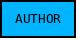
\includegraphics{images/entity.jpeg}}
     & Ορθογώνια: οντότητες. \\ \hline

     \vspace{0.3cm}
     \resizebox*{0.20\textwidth}{!}{
     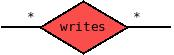
\includegraphics{images/relationship.jpeg}}
     & Ρόμβοι: συσχετίσεις. \\ \hline

     \vspace{0.3cm}
     \resizebox*{0.20\textwidth}{!}{
     
\includegraphics{images/line.jpeg}}
     & Γραμμές: συνδέουν χαρακτηριστικά με οντότητες, οντότητες με συσχετίσεις. \\ \hline

     \vspace{0.3cm}
     %\resizebox*{0.20\textwidth}{!}{
     \center
     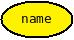
\includegraphics{images/characteristicl.jpeg}%}
     & Ελλείψεις: χαρακτηριστικά. \\ \hline

     \vspace{0.3cm}
     \resizebox*{0.20\textwidth}{!}{
     
\includegraphics{images/characteristicl_many.jpeg}}
     & Διπλές ελλείψεις: πλειότιμα χαρακτηριστικά. \\ \hline

%     \vspace{0.3cm}
     %\resizebox*{0.20\textwidth}{!}{
     \center
%     
\includegraphics{images/characteristicl_many.jpeg}}
%     & Διακεκομμένες ελλείψεις: εξαρτημένα χαρακτηριστικά. \\ \hline

     \vspace{0.3cm}
     %\resizebox*{0.20\textwidth}{!}{
     \center
     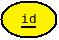
\includegraphics{images/key.jpeg}%}
     & Υπογραμμίσεις: πρωτεύοντα κλειδιά. \\ \hline

     \vspace{0.3cm}
     \resizebox*{0.20\textwidth}{!}{
     
\includegraphics{images/entity_weak.jpeg}}
     & Διπλό ορθογώνιο: Αδύναμο σύνολο οντοτήτων. \\ \hline

     \vspace{0.3cm}
     \resizebox*{0.20\textwidth}{!}{
     
\includegraphics{images/isa.jpeg}}
     & Τρίγωνο: Εξιδίκευση. \\ \hline
  \end{tabular}
\caption{Τα εικονίδια του διαγράμματος οντοτήτων συσχετίσεων.}
\label{table:icons}
\end{center}
\end{table}


%\begin{landscape}
\begin{figure}
\begin{center}
\resizebox*{!}{\textwidth}{
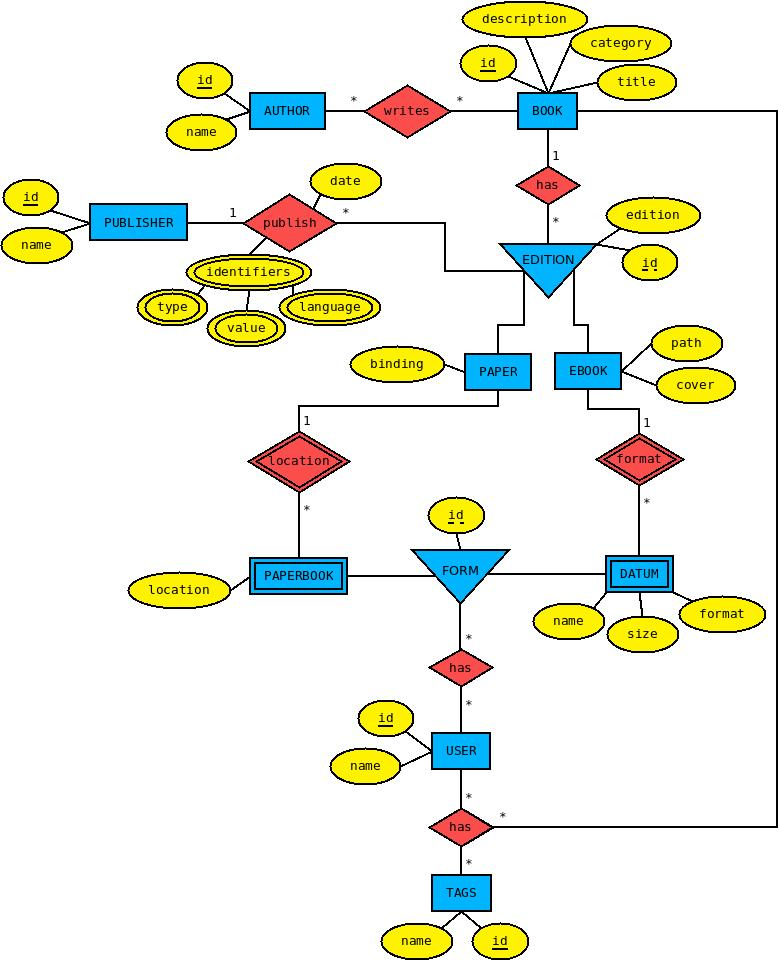
\includegraphics{images/ERDiagram.jpeg}}
\caption{Διάγραμμα οντοτήτων - συσχετίσεων}
\label{fig:ER:diagram}
\end{center}
\end{figure}
%\end{landscape}

\subsubsection{Σχολιασμός οντοτήτων και σχέσεων της βάσης δεδομένων}
\begin{itemize}
  \item Η οντότητα FORM θα μπορούσε να είχε παραληφθεί και να είχαν δημιουργηθεί απευθείας σχέσεις μεταξύ των χρηστών και των paperbook και datum αντίστοιχα. 
  \item Για τις οντότητες AUTHOR, PUBLISHER, USER τα χαρακτηριστικά που υπάρχουν είναι λίγα. Για την κάθε οντότητα θα μπορούσαν να καταγραφούν και άλλες λεπτομέρειες (όπως ημερομηνία γέννησης για τους συγγραφείς, κ.λ.π.) αλλά θεωρήθηκε σκόπιμα να μην συμπεριληφθούν αφού αυτές οι λεπτομέρειες δεν επηρεάζουν τον γενικό σχεδιασμό της βάσης και κάνουν πιο εύκολη την υλοποίηση της βάσης σε αυτό το επίπεδο. 
\end{itemize}


\subsection{Λογικός σχεδιασμός}

Ο λογικός σχεδιασμός είναι η διαδικασία μετατροπής ενός εννοιολογικού μοντέλου (διαισθητικής περιγραφής) σε τυπικά σχήματα εκφρασμένα στο επιλεγμένο (υποστηριζόμενο από το ΣΔΒΔ) μοντέλο δεδομένων (π.χ. Σχεσιακό μοντέλο) \cite{class_notes}.

\subsection{Μετατροπή μοντέλου οντοτήτων - συσχετίσεων σε σχεσιακό σχή\-μα}

Οι κανόνες που χρησιμοποιούνται για την μετατροπή του μοντέλου οντοτήτων - συσχετίσεων σε σχεσιακό σχήμα φαίνονται παρακάτω \cite{class_notes}:

\begin{description}

  \item[Οντότητες:] Ένα ισχυρό σύνολο οντοτήτων μετατρέπεται σε πίνακα (με τα ίδια χαρακτηριστικά). Ένα αδύναμο σύνολο οντοτήτων γίνεται πίνακας που περιλαμβάνει μια στήλη για το πρωτεύον κλειδί του ισχυρότερου συνόλου οντοτήτων που το ταυτοποιεί. 
  \item[Συσχετίσεις 1:1 :] Οι συσχετίσεις 1:1 μπορούν να αναπαρασταθούν είτε προσθέτοντας το πρωτεύον κλειδί της μία πλευράς ως επιπλέον χαρακτηριστικό στον πίνακα της άλλη πλευράς είτε δημιουργώντας ένα νέο πίνακα που έχει τα κλειδιά των δύο πινάκων.
  \item[Συσχετίσεις 1:Ν :] Οι συσχετίσεις 1:Ν μπορούν να αναπαρασταθούν απλά με την προσθήκη ενός επιπλέον χαρακτηριστικού στην πλευρά Ν (το πρωτεύον κλειδί τις πλευράς 1). Εάν η συμμετοχή στην πλευρά Ν είναι μερική, μπορεί να προκύψει μία στήλη που να έχει πολλές κενές τιμές. Οπότε η δημιουργία ενός νέου πίνακα μπορεί να συμφέρει.
  \item[Συσχετίσεις Μ:Ν :] Ένα σύνολο συσχετίσεων M:N αναπαριστάται ως πίνακας με στήλες για τα πρωτεύοντα κλειδιά των οντοτήτων που συμμετέχουν, και επιπλέον όλα τα χαρακτηριστικά του συνόλου συσχετίσεων. 
  \item[Σύνθετα χαρακτηριστικά :] Τα σύνθετα χαρακτηριστικά μετατρέπονται σε ένα σύνολο απλών.
  \item[Πλειότιμα χαρακτηριστικά :] Από τα πλειότιμα χαρακτηριστικά ενός συνόλου οντοτήτων προκύπτει νέος πίνακας. Ο πίνακας αυτός έχεις ως στήλες το πρωτεύον κλειδί του συνόλου οντοτήτων και μία ακόμα που αντιστοιχεί στο πλειότιμο χαρακτηριστικό.
  \item[Εξειδίκευση :] Όταν έχουμε εξειδίκευση, τότε προκύπτει ένας πίνακας για κάθε εμπλεκόμενο σύνολο οντοτήτων, όπου καθένας από τους πίνακες εξειδίκευσης συμπεριλαμβάνει ως στήλη το πρωτεύον κλειδί του πίνακα γενίκευσης.
 
\end{description}

Ακολουθώντας τους παραπάνω κανόνες προκύπτει το σχήμα \ref{fig:RelationalModel:diagram}.

\begin{landscape}
\begin{figure}
\begin{center}
\resizebox*{23.5cm}{!}{
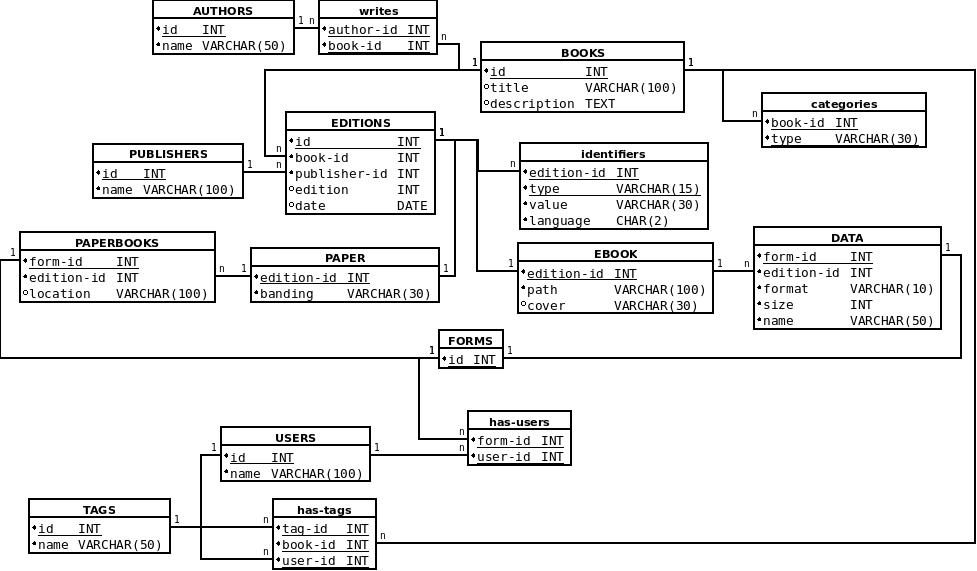
\includegraphics{images/RelationalModel.jpeg}}
\caption{Σχεσιακό σχήμα}
\label{fig:RelationalModel:diagram}
\end{center}
\end{figure}
\end{landscape}


\begin{landscape}
\subsubsection{Ανάλυση πινάκων}
\label{table_analysis}

\begin{table}[htbp]
\begin{center}
  \begin{tabular}{|c|c|m{0.35\textwidth}|m{0.35\textwidth}|m{2.0cm}|c|m{1.5cm}|}
    \hline
    {\bf Πεδίο} & {\bf Τύπος μεταβλητής} & {\bf Εύρος τιμών} & {\bf Περιγραφή} & {\bf Πρωτεύον κλειδί} & {\bf Null} & {\bf Ξένο κλειδί} \\ \hline
    id & INT UNSIGNED & 0 έως 4294967295 & Μοναδικός αριθμός που χρησιμεύει ως πρωτεύον κλειδί & ΝΑΙ & ΟΧΙ & ΟΧΙ \\ \hline
    title & VARCHAR(100) & Όλα τα Αλφαριθμητικά ως 100 χαρακτήρες & Ο τίτλος του βιβλίου & ΟΧΙ & ΟΧΙ & ΟΧΙ \\ \hline
    descritpion & TEXT & Όλα τα Αλφαριθμητικά & Μία περιγραφή του βιβλίου & ΟΧΙ & ΟΧΙ & ΟΧΙ \\ \hline
  \end{tabular}
\caption{Ο πίνακας books.}
\label{table:db_table:books}
\end{center}
\end{table}

Ο πίνακας books (βλ. πίνακα \ref{table:db_table:books}) όπως ειπώθηκε και στην ενότητα \ref{ERmodel} αποτυπώνει τις γενικές πληροφορίες για τα βιβλία. Περιέχει το μοναδικό εσωτερικό αριθμό που χρησιμοποιείται από την βάση δεδομένων ως πρωτεύον κλειδί ενώ ακόμα περιέχει και τον τίτλο του βιβλίου καθώς και μία περιγραφή για το βιβλίο. Για το πρωτεύον αριθμό χρησιμοποιείται ένας ακέραιος αριθμός ενώ για τα υπόλοιπα πεδία χρησιμοποιούνται διάφορου μήκους αλφαριθμητικά. 
\end{landscape}

\begin{landscape}
\begin{table}[htbp]
\begin{center}
  \begin{tabular}{|c|c|m{0.35\textwidth}|m{0.35\textwidth}|m{2.0cm}|c|m{1.5cm}|}
    \hline
    {\bf Πεδίο} & {\bf Τύπος μεταβλητής} & {\bf Εύρος τιμών} & {\bf Περιγραφή} & {\bf Πρωτεύον κλειδί} & {\bf Null} & {\bf Ξένο κλειδί} \\ \hline
    book-id & INT UNSIGNED & 0 έως 4294967295 & Ξένο κλειδί του πίνακα. Χρησιμοποιείται για την υλοποίηση μίας 1:N σχέσης με τον πίνακα books & ΝΑΙ & ΟΧΙ & NAI \\ \hline
    type & VARCHAR(30) & Όλα τα Αλφαριθμητικά ως 15 χαρακτήρες & Περιγράφει την κατηγορία στην οποία ανήκει το βιβλίο & ΝΑΙ & ΟΧΙ & ΟΧΙ \\ \hline
  \end{tabular}
\caption{Ο πίνακας categories.}
\label{table:db_table:categories}
\end{center}
\end{table}

Ο πίνακας categories (βλ. πίνακα \ref{table:db_table:categories}) αποτυπώνει το πλειότιμο χαρακτηριστικό categories. Ένα βιβλίο μπορεί να ανήκει σε πολλές κατηγορίες και γι` αυτό το σκοπό δημιουργείται ένα επιπλέον πίνακας για να αποθηκεύονται σε αυτόν όλες οι δυνατές τιμές. Το πρωτεύον κλειδί του πίνακα είναι σύνθετο και αποτελείται από το book-id (που είναι ταυτόχρονα και ξένο κλειδί που αποτυπώνει την σύνδεση με τον πίνακα books) και από το type (το οποίο αποτυπώνει την κατηγορία του βιβλίου). 
\end{landscape}

\begin{landscape}
\begin{table}[htbp]
\begin{center}
  \begin{tabular}{|c|c|m{0.35\textwidth}|m{0.35\textwidth}|m{2.0cm}|c|m{1.5cm}|}
    \hline
    {\bf Πεδίο} & {\bf Τύπος μεταβλητής} & {\bf Εύρος τιμών} & {\bf Περιγραφή} & {\bf Πρωτεύον κλειδί} & {\bf Null} & {\bf Ξένο κλειδί} \\ \hline
    id & INT UNSIGNED & 0 έως 4294967295 & Μοναδικός αριθμός που χρησιμεύει ως πρωτεύον κλειδί & ΝΑΙ & ΟΧΙ & ΟΧΙ \\ \hline
    book-id & INT UNSIGNED & 0 έως 4294967295 & Ξένο κλειδί του πίνακα. Χρησιμοποιείται για την υλοποίηση μίας 1:N σχέσης με τον πίνακα books & ΟΧΙ & ΟΧΙ & NAI \\ \hline
    publisher-id & INT UNSIGNED & 0 έως 4294967295 & Ξένο κλειδί του πίνακα. Χρησιμοποιείται για την υλοποίηση μίας 1:N σχέσης με τον πίνακα  & ΟΧΙ & ΟΧΙ & NAI \\ \hline
    edition & INT UNSIGNED & 0 έως 4294967295 & Αριθμός που δείχνει την έκδοση του βιβλίου  & ΟΧΙ & ΝΑΙ & ΟΧΙ \\ \hline
    date & DATE & 1000-01-01 έως 9999-12-31 & Ημερομηνία έκδοσης του βιβλίου & OXI & ΝΑΙ & ΟΧΙ \\ \hline
  \end{tabular}
\caption{Ο πίνακας editions.}
\label{table:db_table:editions}
\end{center}
\end{table}

Ο πίνακας editions (βλ. πίνακα \ref{table:db_table:editions}) αποτυπώνει τις εκδόσεις που υπάρχουν για τα βιβλία του πίνακα books. Μία διαφορετική έκδοση ενός βιβλίου μπορεί να υπάρχει για πολλούς λόγους, όπως να υπάρχει διαφορετικός εκδότης ή να έχει επανεκδοθεί το βιβλίο κ.λ.π. . Ο πίνακας αυτός περιέχει το μοναδικό εσωτερικό αριθμό που χρησιμοποιείται από την βάση δεδομένων ως πρωτεύον κλειδί για να ξεχωρίζει τις εκδόσεις των βιβλίων. Ακόμα περιέχει δύο ακόμα ακεραίους (το book-id και το publisher-id) οι οποίοι χρησιμοποιούνται ως ξένα κλειδιά για να συνδεθούν με τους πίνακες books και publishers. Τέλος περιέχει τον αριθμό της έκδοσης και την ημερομηνία έκδοσης της συγκεκριμένης έκδοσης.
\end{landscape}

\begin{landscape}
\begin{table}[htbp]
\begin{center}
  \begin{tabular}{|c|c|m{0.35\textwidth}|m{0.35\textwidth}|m{2.0cm}|c|m{1.5cm}|}
    \hline
    {\bf Πεδίο} & {\bf Τύπος μεταβλητής} & {\bf Εύρος τιμών} & {\bf Περιγραφή} & {\bf Πρωτεύον κλειδί} & {\bf Null} & {\bf Ξένο κλειδί} \\ \hline
    edition-id & INT UNSIGNED & 0 έως 4294967295 & Ξένο κλειδί του πίνακα. Χρησιμοποιείται για την υλοποίηση μίας 1:Μ σχέσης με τον πίνακα books & ΝΑΙ & ΟΧΙ & NAI \\ \hline
    type & VARCHAR(15) & Όλα τα Αλφαριθμητικά ως 15 χαρακτήρες & Περιγράφει το είδος του αναγνωριστικού του βιβλίου (ISBN, amazon id, κ.λ.π.)  & ΝΑΙ & ΟΧΙ & ΟΧΙ \\ \hline
    value & VARCHAR(30) & Όλα τα Αλφαριθμητικά ως 30 χαρακτήρες & Η τιμή του αναγνωριστικού  & OXI & ΟΧΙ & ΟΧΙ \\ \hline
    language & VARCHAR(2) & Όλα τα Αλφαριθμητικά ως 2 χαρακτήρες & Συντομογραφία της γλώσσας στην οποία είναι γραμμένο το βιβλίο  & OXI & ΟΧΙ & ΟΧΙ \\ \hline
  \end{tabular}
\caption{Ο πίνακας identifiers.}
\label{table:db_table:identifiers}
\end{center}
\end{table}

Ο πίνακας identifiers (βλ. πίνακα \ref{table:db_table:identifiers}) αποτυπώνει το πλειότιμο χαρακτηριστικό της σχέσης publish. Μία συγκεκριμένη έκδοση ενός βιβλίου μπορεί να περιέχει πολλά αναγνωριστικά όπως isbn 10 ψηφίων, isbn 13 ψηφίων καθώς και άλλα αναγνωριστικά που αποδίδονται από διάφορες εταιρείες όπως η google και η amazon. Γι` αυτό το σκοπό δημιουργήθηκε ο συγκεκριμένος πίνακας για να αποτυπώσει τις συγκεκριμένες πληροφορίες. Το πρωτεύον κλειδί του πίνακα είναι σύνθετο και αποτελείται από το edition-id (που είναι ταυτόχρονα και ξένο κλειδί που αποτυπώνει την σύνδεση με τον πίνακα editions) και από το type (Αυτό συμβαίνει διότι το ίδιο αναγνωριστικό (π.χ. το isbn 13 χαρακτήρων) δεν μπορεί να έχει δύο διαφορετικές τιμές για την ίδια έκδοση του βιβλίου). Ακόμα καταγράφεται η τιμή του αναγνωριστικού καθώς και η γλώσσα στην οποία είναι γραμμένη η συγκεκριμένη έκδοση του βιβλίου.
\end{landscape}


\begin{landscape}
\begin{table}[htbp]
\begin{center}
  \begin{tabular}{|c|c|m{0.35\textwidth}|m{0.35\textwidth}|m{2.0cm}|c|m{1.5cm}|}
    \hline
    {\bf Πεδίο} & {\bf Τύπος μεταβλητής} & {\bf Εύρος τιμών} & {\bf Περιγραφή} & {\bf Πρωτεύον κλειδί} & {\bf Null} & {\bf Ξένο κλειδί} \\ \hline
    edition-id & INT UNSIGNED & 0 έως 4294967295 & Ξένο κλειδί του πίνακα. Χρησιμοποιείται για την υλοποίηση μίας 1:1 σχέσης με τον πίνακα books & ΝΑΙ & ΟΧΙ & NAI \\ \hline
    banding & VARCHAR(30) & Όλα τα Αλφαριθμητικά ως 30 χαρακτήρες & Η τιμή του αναγνωριστικού  & OXI & ΟΧΙ & ΟΧΙ \\ \hline
  \end{tabular}
\caption{Ο πίνακας paper.}
\label{table:db_table:paper}
\end{center}
\end{table}

Ο πίνακας paper (βλ. πίνακα \ref{table:db_table:paper}) είναι πίνακας ειδίκευσης ο οποίος αποτυπώνει τις επιπλέον πληροφορίες που χρειάζονται οι έντυπες εκδόσεις. Συγκεκριμένα το είδος του εξωφύλλου (αν είναι σκληρό, χάρτινο, κ.λ.π.). Ακόμα περιέχει και το edition-id το οποίο είναι ταυτόχρονα πρωτεύον και ξένο κλειδί που ενώνει τον συγκεκριμένο πίνακα με τον πίνακα editions.
\end{landscape}

\begin{landscape}
\begin{table}[htbp]
\begin{center}
  \begin{tabular}{|c|c|m{0.35\textwidth}|m{0.35\textwidth}|m{2.0cm}|c|m{1.5cm}|}
    \hline
    {\bf Πεδίο} & {\bf Τύπος μεταβλητής} & {\bf Εύρος τιμών} & {\bf Περιγραφή} & {\bf Πρωτεύον κλειδί} & {\bf Null} & {\bf Ξένο κλειδί} \\ \hline
    edition-id & INT UNSIGNED & 0 έως 4294967295 & Ξένο κλειδί του πίνακα. Χρησιμοποιείται για την υλοποίηση μίας 1:1 σχέσης με τον πίνακα books & ΝΑΙ & ΟΧΙ & NAI \\ \hline
    path & VARCHAR(100) &  Όλα τα Αλφαριθμητικά ως 100 χαρακτήρες & Το path στο οποίο είναι αποθηκευμένα τα αρχεία των ηλεκτρονικών βιβλίων & OXI & ΟΧΙ & ΟΧΙ \\ \hline
    cover & VARCHAR(30) &  Όλα τα Αλφαριθμητικά ως 30 χαρακτήρες & Το path στο οποίο είναι αποθηκευμένο το εξώφυλλο των ηλεκτρονικών βιβλίων & OXI & ΟΧΙ & ΟΧΙ \\ \hline
  \end{tabular}
\caption{Ο πίνακας ebook.}
\label{table:db_table:ebook}
\end{center}
\end{table}

Ο πίνακας ebook (βλ. πίνακα \ref{table:db_table:ebook}) είναι ομοίως με τον πίνακα paper ένας πίνακας ειδίκευσης ο οποίος αποτυπώνει τις επιπλέον πληροφορίες που χρειάζονται οι ηλεκτρονικές εκδόσεις. Συγκεκριμένα αποθηκεύει το path στο οποίο είναι αποθηκευμένα τα αρχεία των ηλεκτρονικών βιβλίων καθώς το όνομα του αρχείου του εξωφύλλου του βιβλίου. Ομοίως περιέχει και το edition-id το οποίο είναι ταυτόχρονα πρωτεύον και ξένο κλειδί που ενώνει τον συγκεκριμένο πίνακα με τον πίνακα editions. 
\end{landscape}

\begin{landscape}
\begin{table}[htbp]
\begin{center}
  \begin{tabular}{|c|c|m{0.35\textwidth}|m{0.35\textwidth}|m{2.0cm}|c|m{1.5cm}|}
    \hline
    {\bf Πεδίο} & {\bf Τύπος μεταβλητής} & {\bf Εύρος τιμών} & {\bf Περιγραφή} & {\bf Πρωτεύον κλειδί} & {\bf Null} & {\bf Ξένο κλειδί} \\ \hline
    id & INT UNSIGNED & 0 έως 4294967295 & Μοναδικός αριθμός που χρησιμεύει ως πρωτεύον κλειδί & ΝΑΙ & ΟΧΙ & ΟΧΙ \\ \hline
    name & VARCHAR(100) & Όλα τα Αλφαριθμητικά ως 100 χαρακτήρες & Ο τίτλος του εκδότη & ΟΧΙ & ΟΧΙ & ΟΧΙ \\ \hline
  \end{tabular}
\caption{Ο πίνακας publishers.}
\label{table:db_table:publishers}
\end{center}
\end{table}

Ο πίνακας publishers (βλ. πίνακα \ref{table:db_table:publishers}) περιέχει τις πληροφορίες για τους εκδότες. Περιέχει το μοναδικό εσωτερικό αριθμό που χρησιμοποιείται από την βάση δεδομένων ως πρωτεύον κλειδί ενώ ακόμα περιέχει και το όνομα του εκδότη. Για το πρωτεύον κλειδί χρησιμοποιείται ένας ακέραιος αριθμός ενώ για το όνομα χρησιμοποιείται αλφαριθμητικό.
\end{landscape}




\begin{landscape}
\begin{table}[htbp]
\begin{center}
  \begin{tabular}{|c|c|m{0.35\textwidth}|m{0.35\textwidth}|m{2.0cm}|c|m{1.5cm}|}
    \hline
    {\bf Πεδίο} & {\bf Τύπος μεταβλητής} & {\bf Εύρος τιμών} & {\bf Περιγραφή} & {\bf Πρωτεύον κλειδί} & {\bf Null} & {\bf Ξένο κλειδί} \\ \hline
    id & INT UNSIGNED & 0 έως 4294967295 & Μοναδικός αριθμός που χρησιμεύει ως πρωτεύον κλειδί & ΝΑΙ & ΟΧΙ & ΟΧΙ \\ \hline
    name & VARCHAR(50) & Όλα τα Αλφαριθμητικά ως 50 χαρακτήρες & Το όνομα του συγγραφέα & ΟΧΙ & ΟΧΙ & ΟΧΙ \\ \hline
  \end{tabular}
\caption{Ο πίνακας authors.}
\label{table:db_table:authors}
\end{center}
\end{table}

Ο πίνακας authors (βλ. πίνακα \ref{table:db_table:authors}) περιέχει τις πληροφορίες για τους συγγραφείς. Περιέχει το μοναδικό εσωτερικό αριθμό που χρησιμοποιείται από την βάση δεδομένων ως πρωτεύον κλειδί ενώ ακόμα περιέχει και το όνομα του συγγραφέα. Για το πρωτεύον κλειδί χρησιμοποιείται ένας ακέραιος αριθμός ενώ για το όνομα χρησιμοποιείται αλφαριθμητικό.
\\
%\end{landscape}

%\begin{landscape}
\begin{table}[htbp]
\begin{center}
  \begin{tabular}{|c|c|m{0.35\textwidth}|m{0.35\textwidth}|m{2.0cm}|c|m{1.5cm}|}
    \hline
    {\bf Πεδίο} & {\bf Τύπος μεταβλητής} & {\bf Εύρος τιμών} & {\bf Περιγραφή} & {\bf Πρωτεύον κλειδί} & {\bf Null} & {\bf Ξένο κλειδί} \\ \hline
    author-id & INT UNSIGNED & 0 έως 4294967295 & Ξένο κλειδί του πίνακα. Χρησιμοποιείται για την υλοποίηση μίας 1:Μ σχέσης με τον πίνακα authors & ΝΑΙ & ΟΧΙ & NAI \\ \hline
    book-id & INT UNSIGNED & 0 έως 4294967295 & Ξένο κλειδί του πίνακα. Χρησιμοποιείται για την υλοποίηση μίας 1:Μ σχέσης με τον πίνακα books & ΝΑΙ & ΟΧΙ & NAI \\ \hline
  \end{tabular}
\caption{Ο πίνακας writes.}
\label{table:db_table:writes}
\end{center}
\end{table}

Ο πίνακας writes (βλ. πίνακα \ref{table:db_table:writes}) αποτυπώνει την σχέση Μ:Ν μεταξύ του πίνακα authors και books. Το πρωτεύον κλειδί του πίνακα είναι σύνθετο και αποτελείται από το book-id και το author-id που είναι ταυτόχρονα ξένα κλειδιά για τους πίνακες books και authors αντίστοιχα.

\end{landscape}

\begin{landscape}
\begin{table}[htbp]
\begin{center}
  \begin{tabular}{|c|c|m{0.35\textwidth}|m{0.35\textwidth}|m{2.0cm}|c|m{1.5cm}|}
    \hline
    {\bf Πεδίο} & {\bf Τύπος μεταβλητής} & {\bf Εύρος τιμών} & {\bf Περιγραφή} & {\bf Πρωτεύον κλειδί} & {\bf Null} & {\bf Ξένο κλειδί} \\ \hline
    form-id & INT UNSIGNED & 0 έως 4294967295 & Μοναδικός αριθμός που χρησιμεύει ως πρωτεύον κλειδί & ΝΑΙ & ΟΧΙ & ΟΧΙ \\ \hline
    edition-id & INT UNSIGNED & 0 έως 4294967295 & Ξένο κλειδί του πίνακα. Χρησιμοποιείται για την υλοποίηση μίας 1:Ν σχέσης με τον πίνακα paper & OXI & ΟΧΙ & NAI \\ \hline
    location & VARCHAR(100) &  Όλα τα Αλφαριθμητικά ως 100 χαρακτήρες & Πεδίο που περιγράφει την φυσική τοποθεσία του βιβλίου & OXI & ΟΧΙ & ΟΧΙ \\ \hline
  \end{tabular}
\caption{Ο πίνακας paperbook.}
\label{table:db_table:paperbook}
\end{center}
\end{table}

Ο πίνακας paperbook (βλ. πίνακας \ref{table:db_table:paperbook}) είναι ένας πίνακας ειδίκευσης ο οποίος αποτυπώνει την φυσική μορφή των έντυπων βιβλίων. Για ένα βιβλίο μπορεί οι χρήστες να έχουν πολλά αντίτυπα. Επομένως αυτά τα αντίτυπα καταγράφονται σε αυτά τον πίνακα. Ως πρωτεύον κλειδί χρησιμοποιείται ένας ακέραιος αριθμός, ενώ ακόμα υπάρχουν σε αυτό τον πίνακα το edition-id που χρησιμεύει ως ξένο κλειδί για την υλοποίηση της σχέσης με τον πίνακα editions. Τέλος καταγράφεται ακόμα η φυσική τοποθεσία του αντιτύπου.
\end{landscape}

\begin{landscape}
\begin{table}[htbp]
\begin{center}
  \begin{tabular}{|c|c|m{0.35\textwidth}|m{0.35\textwidth}|m{2.0cm}|c|m{1.5cm}|}
    \hline
    {\bf Πεδίο} & {\bf Τύπος μεταβλητής} & {\bf Εύρος τιμών} & {\bf Περιγραφή} & {\bf Πρωτεύον κλειδί} & {\bf Null} & {\bf Ξένο κλειδί} \\ \hline
    form-id & INT UNSIGNED & 0 έως 4294967295 & Μοναδικός αριθμός που χρησιμεύει ως πρωτεύον κλειδί & ΝΑΙ & ΟΧΙ & ΟΧΙ \\ \hline
    edition-id & INT UNSIGNED & 0 έως 4294967295 & Ξένο κλειδί του πίνακα. Χρησιμοποιείται για την υλοποίηση μίας 1:Ν σχέσης με τον πίνακα books & ΟΧΙ & ΟΧΙ & NAI \\ \hline
    format & VARCHAR(10) &  Όλα τα Αλφαριθμητικά ως 100 χαρακτήρες & Πεδίο που περιγράφει το format του ηλεκτρονικού βιβλίου & OXI & ΟΧΙ & ΟΧΙ \\ \hline
    size & INT UNSIGNED & 0 έως 4294967295 & Πεδίο που περιγράφει το μέγεθος του ηλεκτρονικού βιβλίου σε bytes & OXI & ΟΧΙ & ΟΧΙ \\ \hline
    name & VARCHAR(50) &  Όλα τα Αλφαριθμητικά ως 50 χαρακτήρες & Πεδίο που περιγράφει το όνομα του αρχείου του ηλεκτρονικού βιβλίου & OXI & ΟΧΙ & ΟΧΙ \\ \hline
  \end{tabular}
\caption{Ο πίνακας data.}
\label{table:db_table:data}
\end{center}
\end{table}

Ο πίνακας data (βλ. πίνακας \ref{table:db_table:data}) είναι ομοίως ένας πίνακας ειδίκευσης ο οποίος αποτυπώνει την ηλεκτρονική μορφή των \en{ebooks}). Για ένα ηλεκτρονικό βιβλίο καταγράφεται το format στο οποίο είναι αποθηκευμένο (epub, pdf, κ.λ.π.), το μέγεθος του αρχείου και το όνομα του αρχείου
\end{landscape}

\begin{landscape}
\begin{table}[htbp]
\begin{center}
  \begin{tabular}{|c|c|m{0.35\textwidth}|m{0.35\textwidth}|m{2.0cm}|c|m{1.5cm}|}
    \hline
    {\bf Πεδίο} & {\bf Τύπος μεταβλητής} & {\bf Εύρος τιμών} & {\bf Περιγραφή} & {\bf Πρωτεύον κλειδί} & {\bf Null} & {\bf Ξένο κλειδί} \\ \hline
    id & INT UNSIGNED & 0 έως 4294967295 & Μοναδικός αριθμός που χρησιμεύει ως πρωτεύον κλειδί & ΝΑΙ & ΟΧΙ & ΟΧΙ \\ \hline
  \end{tabular}
\caption{Ο πίνακας forms.}
\label{table:db_table:forms}
\end{center}
\end{table}

Ο πίνακας forms (βλ. πίνακα \ref{table:db_table:forms}) είναι ο πίνακας ο οποίος εξειδικεύεται στο  paperbooks και στο data. Ο κύριος λόγος ύπαρξης του είναι για να μην υπάρχουν δύο πίνακες για να υλοποιούν την σχέση μεταξύ των χρηστών και την φυσική μορφή των βιβλίων (είτε είναι έντυπο βιβλίο είτε σε ηλεκτρονική μορφή). Ο πίνακας αυτός περιέχει μόνο το πρωτεύον κλειδί το οποίο χρησιμοποιείται και στους πίνακες είδικευσης. Εναλλακτικά θα μπορούσαν να είχαν δημιουργηθεί στην θέση του δύο πίνακες η οποίοι θα υλοποίσαν την σχέση Μ:Ν μεταξύ των χρηστών και των πινάκων paperbooks και data.
\end{landscape}


\begin{landscape}
\begin{table}[htbp]
\begin{center}
  \begin{tabular}{|c|c|m{0.35\textwidth}|m{0.35\textwidth}|m{2.0cm}|c|m{1.5cm}|}
    \hline
    {\bf Πεδίο} & {\bf Τύπος μεταβλητής} & {\bf Εύρος τιμών} & {\bf Περιγραφή} & {\bf Πρωτεύον κλειδί} & {\bf Null} & {\bf Ξένο κλειδί} \\ \hline
    id & INT UNSIGNED & 0 έως 4294967295 & Μοναδικός αριθμός που χρησιμεύει ως πρωτεύον κλειδί & ΝΑΙ & ΟΧΙ & ΟΧΙ \\ \hline
    name & VARCHAR(100) & Όλα τα Αλφαριθμητικά ως 100 χαρακτήρες & Το όνομα του χρήστη & ΟΧΙ & ΟΧΙ & ΟΧΙ \\ \hline
  \end{tabular}
\caption{Ο πίνακας users.}
\label{table:db_table:users}
\end{center}
\end{table}

Ο πίνακας users (βλ. πίνακα \ref{table:db_table:users}) περιέχει τις πληροφορίες για τους χρήστες. Περιέχει το μοναδικό εσωτερικό αριθμό που χρησιμοποιείται από την βάση δεδομένων ως πρωτεύον κλειδί ενώ ακόμα περιέχει και το όνομα του χρήστη. Για το πρωτεύον κλειδί χρησιμοποιείται ένας ακέραιος αριθμός ενώ για το όνομα χρησιμοποιείται αλφαριθμητικό. \\
%\end{landscape}

%\begin{landscape}
\begin{table}[htbp]
\begin{center}
  \begin{tabular}{|c|c|m{0.35\textwidth}|m{0.35\textwidth}|m{2.0cm}|c|m{1.5cm}|}
    \hline
    {\bf Πεδίο} & {\bf Τύπος μεταβλητής} & {\bf Εύρος τιμών} & {\bf Περιγραφή} & {\bf Πρωτεύον κλειδί} & {\bf Null} & {\bf Ξένο κλειδί} \\ \hline
    form-id & INT UNSIGNED & 0 έως 4294967295 & Ξένο κλειδί του πίνακα. Χρησιμοποιείται για την υλοποίηση μίας 1:Μ σχέσης με τον πίνακα books & ΝΑΙ & ΟΧΙ & NAI \\ \hline
    user-id & INT UNSIGNED & 0 έως 4294967295 & Ξένο κλειδί του πίνακα. Χρησιμοποιείται για την υλοποίηση μίας 1:Μ σχέσης με τον πίνακα users & ΝΑΙ & ΟΧΙ & NAI \\ \hline
  \end{tabular}
\caption{Ο πίνακας has-users.}
\label{table:db_table:has-users}
\end{center}
\end{table}

Ο πίνακας has-users (βλ. πίνακα \ref{table:db_table:has-users}) αποτυπώνει την σχέση Μ:Ν μεταξύ του πίνακα forms και users. Το πρωτεύον κλειδί του πίνακα είναι σύνθετο και αποτελείται από το form-id και το user-id που είναι ταυτόχρονα ξένα κλειδιά για τους πίνακες  forms και users αντίστοιχα. Ο πίνακας αυτός αποτυπώνει την "ιδιοκτησία των βιλβίων", δηλαδή σε ποιους χρήστες ανήκουν ποια βιβλία.
\end{landscape}

\begin{landscape}
\begin{table}[htbp]
\begin{center}
  \begin{tabular}{|c|c|m{0.35\textwidth}|m{0.35\textwidth}|m{2.0cm}|c|m{1.5cm}|}
    \hline
    {\bf Πεδίο} & {\bf Τύπος μεταβλητής} & {\bf Εύρος τιμών} & {\bf Περιγραφή} & {\bf Πρωτεύον κλειδί} & {\bf Null} & {\bf Ξένο κλειδί} \\ \hline
    id & INT UNSIGNED & 0 έως 4294967295 & Μοναδικός αριθμός που χρησιμεύει ως πρωτεύον κλειδί & ΝΑΙ & ΟΧΙ & ΟΧΙ \\ \hline
    name & VARCHAR(50) & Όλα τα Αλφαριθμητικά ως 50 χαρακτήρες & Το όνομα του tag & ΟΧΙ & ΟΧΙ & ΟΧΙ \\ \hline
  \end{tabular}
\caption{Ο πίνακας tags.}
\label{table:db_table:tags}
\end{center}
\end{table}

Ο πίνακας tags (βλ. πίνακα \ref{table:db_table:tags}) περιέχει τις πληροφορίες για τους tags που χρησιμοποιούν οι χρήστες. Περιέχει το μοναδικό εσωτερικό αριθμό που χρησιμοποιείται από την βάση δεδομένων ως πρωτεύον κλειδί ενώ ακόμα περιέχει και το όνομα του tag. Για το πρωτεύον κλειδί χρησιμοποιείται ένας ακέραιος αριθμός ενώ για το όνομα χρησιμοποιείται αλφαριθμητικό. \\
\end{landscape}

\begin{landscape}
\begin{table}[htbp]
\begin{center}
  \begin{tabular}{|c|c|m{0.35\textwidth}|m{0.35\textwidth}|m{2.0cm}|c|m{1.5cm}|}
    \hline
    {\bf Πεδίο} & {\bf Τύπος μεταβλητής} & {\bf Εύρος τιμών} & {\bf Περιγραφή} & {\bf Πρωτεύον κλειδί} & {\bf Null} & {\bf Ξένο κλειδί} \\ \hline
    tag-id & INT UNSIGNED & 0 έως 4294967295 & Ξένο κλειδί του πίνακα. Χρησιμοποιείται για την υλοποίηση μίας 1:Μ σχέσης με τον πίνακα tags & ΝΑΙ & ΟΧΙ & NAI \\ \hline
    book-id & INT UNSIGNED & 0 έως 4294967295 & Ξένο κλειδί του πίνακα. Χρησιμοποιείται για την υλοποίηση μίας 1:Μ σχέσης με τον πίνακα books & ΝΑΙ & ΟΧΙ & NAI \\ \hline
    user-id & INT UNSIGNED & 0 έως 4294967295 & Ξένο κλειδί του πίνακα. Χρησιμοποιείται για την υλοποίηση μίας 1:Μ σχέσης με τον πίνακα users & ΝΑΙ & ΟΧΙ & NAI \\ \hline
  \end{tabular}
\caption{Ο πίνακας has-tags.}
\label{table:db_table:has-tags}
\end{center}
\end{table}

Ο πίνακας has-tags (βλ. πίνακα \ref{table:db_table:has-tags}) υλοποιεί την τριμελή σχέση μεταξύ των βιβλίων, των χρηστών και tags. Το πρωτεύον κλειδί του πίνακα είναι σύνθετο και αποτελείται από το tag-id, το book-id και το user-id που είναι ταυτόχρονα ξένα κλειδιά για τους πίνακες  tags, books και users αντίστοιχα. Ο πίνακας αυτός αποτυπώνει τα tags που βάζουν οι χρήστες στα βιβλία.
\end{landscape} 

\subsubsection{Boyce-Codd Κανονική Μορφή}

Η κανονικοποίηση του σχήματος της βάσης δεδομένων αποτελεί βασικό βήμα κατά το σχεδιασμό μίας βάσης. Κύριος στόχος της κανονικοποίησης είναι η κατάργηση του πλεονασμού των δεδομένων, ο οποίος δημιουργεί προβλήματα κατά τις εισαγωγές, διαγραφές και ενημερώσεις δεδομένων. Επιπλέον, απαιτείται περισσότερος χώρος για την αποθήκευση των δεδομένων \cite{baseis_manolopoulos, wiki:normalization}. 

Η κανονικοποίηση στηρίζεται στη θεωρία συναρτησιακών εξαρτήσεων. Μία συναρτησιακή εξάρτηση συμβολίζεται με $X \rightarrow Y$ και δηλώνει ότι το σύνολο χαρακτηριστικών $Y$ είναι συναρτησιακά εξαρτώμενο από το σύνολο χαρακτηριστικών του $X$. Αυτό σημαίνει ότι αν δύο γραμμές του πίνακα έχουν ίδιες τιμές για τα χαρακτηριστικά του $X$, τότε πρέπει να έχουν ίδιες τιμές για τα χαρακτηριστικά του $Y$ \cite{baseis_manolopoulos}.

Οι κανονικές μορφές προκύπτουν με διαδοχικές διασπάσεις των πινάκων της βάσης σε απλούστερους. Η απλούστερη κανονική μορφή είναι η πρώτη κανονική μορφή (1NF), ενώ η πέμπτη κανονική μορφή (5NF) είναι η πλέον περιοριστική. Στην πράξη, οι πίνακες κανονικοποιούνται συνήθως μέχρι την κανονική μορφή Boyce-Codd (BCNF) \cite{baseis_manolopoulos}.

Για να προσδιορίσουμε αν ένας πίνακας βρίσκεται στην κανονική μορφή Boyce-Codd αρκεί να εξετάσουμε όλες τις συναρτησιακές εξαρτήσεις $X \rightarrow Y$ ελέγχοντας αν το $X$ αποτελεί κάποιο κλειδί (πρωτεύον ή εναλλακτικό) του πίνακα. Σε διαφορετική περίπτωση θα πρέπει να προχωρήσουμε σε διάσπαση του πίνακα έτσι ώστε να ικανοποιηθεί η συνθήκη της κανονική μορφής Boyce-Codd \cite{baseis_manolopoulos, wiki:boyce-codd}.

Στο σχήμα μας οι συναρτησιακές εξαρτήσεις είναι οι παρακάτω:
\begin{itemize}
\item $R_1$(\underline{id(books)}, title, description, category)
\item $R_2$(\underline{book-id}, \underline{type})
\item $R_3$(\underline{id(editions)}, book-id, publisher-id, edition, date)
\item $R_4$(\underline{edition-id}, \underline{type}, value, language)
\item $R_5$(\underline{id(publisher)}, name)
\item $R_6$(\underline{id(author)}, name)
\item $R_7$(\underline{author-id}, \underline{book-id})
\item $R_8$(\underline{edition-id(paper)}, banding)
\item $R_9$(\underline{edition-id(ebook)}, path, cover)
\item $R_{10}$(\underline{id(forms)})
\item $R_{11}$(\underline{form-id(paperbooks)}, edition-id, location)
\item $R_{12}$(\underline{form-id(data)}, edition-id, format, size, name)
\item $R_{13}$(\underline{id(users)}, name)
\item $R_{14}$(\underline{form-id}, \underline{user-id})
\item $R_{15}$(\underline{id(tags)}, name)
\item $R_{16}$(\underline{tag-id}, \underline{book-id}, \underline{user-id})
\end{itemize}

Όπως παρατηρούμε σε όλες τις συναρτησιακές εξαρτήσεις τα κλειδιά είναι σωστά ορισμένα οπότε δεν χρειάζεται περαιτέρω διάσπαση των πινάκων της βάσης. Επομένως αφού είναι BCNF τότε είναι και 3NF κανονική μορφή.

\section{Υλοποίηση της Βάσης Δεδομένων}

Σε αυτή την ενότητα περιγράφεται η υλοποίηση της βάσης δεδομένων στο ΣΔΒΔ της MariaDB η οποία είναι ένα fork της MySQL.

\subsection{Δημιουργία ειδικού χρήστη}

Σαν πρώτο βήμα είναι η δημιουργία ειδικού χρήστη για την βάση έτσι ώστε να μην χρησιμοποιούμε συνέχεια τον υπερχρήστη. Για την επίτευξη αυτού του σκοπού πληκτρολογούμε στο terminal τα παρακάτω: 

\begin{minted}{bash}
$ mysql --user=root --password
Enter password: 
\end{minted} 
%%$

Και αφού έχουμε μπει στην βάση δημιουργούμε ένα καινούργιο χρήστη και μία νέα βάση και δίνουμε στον χρήστη την δυνατότητα να την τροποποιεί. Όλα αυτά επιτυγχάνονται με τα παρακάτω:

\begin{minted}[breaklines=true]{mysql}
MariaDB [(none)]> CREATE USER 'book'@'localhost' IDENTIFIED BY 'book_password' ;
MariaDB [(none)]> GRANT USAGE ON *.* TO 'book'@'localhost' IDENTIFIED BY 'book_password' WITH MAX_QUERIES_PER_HOUR 0 MAX_CONNECTIONS_PER_HOUR 0 MAX_UPDATES_PER_HOUR 0 MAX_USER_CONNECTIONS 0 ;
MariaDB [(none)]> CREATE DATABASE `book` CHARACTER SET utf8 COLLATE utf8_general_ci;
MariaDB [(none)]> GRANT ALL PRIVILEGES ON `book`.* TO 'book'@'localhost';
\end{minted}

Ο λόγος για τον οποίο δημιουργούμε έναν καινούργιο χρήστη είναι για λόγους ασφαλείας έτσι ώστε να μην χρησιμοποιούμε συνέχεια τον υπερχρήστη. Ακόμα στην νέα βάση προτιμήθηκε να χρησιμοποιηθεί το utf8 έτσι ώστε η βάση μας να υποστηρίζει και τα ελληνικά. Μετά την δημιουργία του καινούργιου χρήστη ξαναμπαίνουμε στο ΣΔΒΔ χρησιμοποιώντας τον καινούργιο χρήστη:

\begin{minted}{bash}
$ mysql --user=book --password
Enter password: 
\end{minted} 

%%$

Παρατηρούμε ότι στις μόνες βάσεις που έχει πρόσβαση ο συγκεκριμένος χρήστης είναι η βάση που δημιουργήσαμε πριν και η βάση που είναι δημιουργημένη από την MariaDB και περιέχει πληροφορίες για την βάση.

\begin{minted}[breaklines=true]{mysql}
MariaDB [(none)]> show databases;
+--------------------+
| Database           |
+--------------------+
| information_schema |
| book               |
+--------------------+
2 rows in set (0.00 sec)
\end{minted}

Μετά αλλάζουμε την βάση και χρησιμοποιούμε την καινούργια βάση που δημιουργήθηκε (μετά από κάθε εντολή δημιουργίας φαίνεται και η περιγραφή του πίνακα μέσα από την MariaDB):

\begin{minted}[breaklines=true]{mysql}
MariaDB [(none)]> use book;
Database changed
MariaDB [book]> 
\end{minted}


\subsection{Δημιουργία πινάκων}

Ύστερα δημιουργούμε του πίνακες που αναφέραμε αναλυτικά στην ενότητα \ref{table_analysis}. Αυτό επιτυγχάνετε με τις παρακάτω εντολές:

\begin{minted}[breaklines=true]{mysql}
MariaDB [book]> CREATE TABLE books (
    -> id int UNSIGNED NOT NULL AUTO_INCREMENT,
    -> title VARCHAR(100) NOT NULL,
    -> description TEXT NOT NULL,
    -> PRIMARY KEY (id) );
Query OK, 0 rows affected (0.12 sec)

MariaDB [book]> describe books;
+-------------+------------------+------+-----+---------+----------------+
| Field       | Type             | Null | Key | Default | Extra          |
+-------------+------------------+------+-----+---------+----------------+
| id          | int(10) unsigned | NO   | PRI | NULL    | auto_increment |
| title       | varchar(100)     | NO   |     | NULL    |                |
| description | text             | NO   |     | NULL    |                |
+-------------+------------------+------+-----+---------+----------------+
3 rows in set (0.01 sec)
\end{minted}

\begin{minted}[breaklines=true]{mysql}
MariaDB [book]> CREATE TABLE categories (
    -> book_id INT UNSIGNED NOT NULL,
    -> type VARCHAR(30),
    -> PRIMARY KEY (book_id, type) );
Query OK, 0 rows affected (0.06 sec)

MariaDB [book]> describe categories;
+---------+------------------+------+-----+---------+-------+
| Field   | Type             | Null | Key | Default | Extra |
+---------+------------------+------+-----+---------+-------+
| book_id | int(10) unsigned | NO   | PRI | NULL    |       |
| type    | varchar(30)      | NO   | PRI |         |       |
+---------+------------------+------+-----+---------+-------+
2 rows in set (0.00 sec)
\end{minted}


\begin{minted}[breaklines=true]{mysql}
MariaDB [book]> CREATE TABLE categories (
    -> book_id INT UNSIGNED NOT NULL,
    -> type VARCHAR(30),
    -> PRIMARY KEY (book_id,type),
    -> FOREIGN KEY (book_id) REFERENCES books(id) );
Query OK, 0 rows affected (0.05 sec)


MariaDB [book]> describe categories;
+---------+------------------+------+-----+---------+-------+
| Field   | Type             | Null | Key | Default | Extra |
+---------+------------------+------+-----+---------+-------+
| book_id | int(10) unsigned | NO   | PRI | NULL    |       |
| type    | varchar(30)      | NO   | PRI |         |       |
+---------+------------------+------+-----+---------+-------+
2 rows in set (0.02 sec)
\end{minted}

\begin{minted}[breaklines=true]{mysql}
MariaDB [book]> CREATE TABLE writes ( 
    -> author_id INT UNSIGNED NOT NULL, 
    -> book_id INT UNSIGNED NOT NULL, 
    -> PRIMARY KEY (author_id, book_id), 
    -> FOREIGN KEY (book_id) REFERENCES books(id), 
    -> FOREIGN KEY (author_id) REFERENCES authors(id) );
Query OK, 0 rows affected (0.06 sec)

MariaDB [book]> describe writes;
+-----------+------------------+------+-----+---------+-------+
| Field     | Type             | Null | Key | Default | Extra |
+-----------+------------------+------+-----+---------+-------+
| author_id | int(10) unsigned | NO   | PRI | NULL    |       |
| book_id   | int(10) unsigned | NO   | PRI | NULL    |       |
+-----------+------------------+------+-----+---------+-------+
2 rows in set (0.01 sec)
\end{minted}

\begin{minted}[breaklines=true]{mysql}
MariaDB [book]> CREATE TABLE publishers ( 
    -> id INT UNSIGNED NOT NULL AUTO_INCREMENT, 
    -> name VARCHAR(50) NOT NULL, 
    -> PRIMARY KEY (id) );
Query OK, 0 rows affected (0.03 sec)

MariaDB [book]> describe publishers;
+-------+------------------+------+-----+---------+----------------+
| Field | Type             | Null | Key | Default | Extra          |
+-------+------------------+------+-----+---------+----------------+
| id    | int(10) unsigned | NO   | PRI | NULL    | auto_increment |
| name  | varchar(50)      | NO   |     | NULL    |                |
+-------+------------------+------+-----+---------+----------------+
2 rows in set (0.00 sec)

\end{minted}

\begin{minted}[breaklines=true]{mysql}
MariaDB [book]> CREATE TABLE editions ( 
    -> id INT UNSIGNED NOT NULL,
    -> book_id INT UNSIGNED NOT NULL AUTO_INCREMENT, 
    -> publisher_id INT UNSIGNED NOT NULL, 
    -> edition INT UNSIGNED, date DATE, 
    -> PRIMARY KEY (id), 
    -> FOREIGN KEY (book_id) REFERENCES books(id), 
    -> FOREIGN KEY (publisher_id) REFERENCES publishers(id) );
Query OK, 0 rows affected (0.09 sec)

MariaDB [book]> describe editions;
+--------------+------------------+------+-----+---------+----------------+
| Field        | Type             | Null | Key | Default | Extra          |
+--------------+------------------+------+-----+---------+----------------+
| id           | int(10) unsigned | NO   | PRI | NULL    | auto_increment |
| book_id      | int(10) unsigned | NO   | MUL | NULL    |                |
| publisher_id | int(10) unsigned | NO   | MUL | NULL    |                |
| edition      | int(10) unsigned | YES  |     | NULL    |                |
| date         | date             | YES  |     | NULL    |                |
+--------------+------------------+------+-----+---------+----------------+
5 rows in set (0.00 sec)

\end{minted}

\begin{minted}[breaklines=true]{mysql}
MariaDB [book]> CREATE TABLE identifiers ( 
    -> edition_id INT UNSIGNED NOT NULL, 
    -> type VARCHAR(15) NOT NULL, 
    -> value VARCHAR(30) NOT NULL, 
    -> language CHAR(2) NOT NULL, 
    -> PRIMARY KEY (edition_id, type), 
    -> FOREIGN KEY (edition_id) REFERENCES editions(id) );
Query OK, 0 rows affected (0.05 sec)

MariaDB [book]> describe identifiers;
+------------+------------------+------+-----+---------+-------+
| Field      | Type             | Null | Key | Default | Extra |
+------------+------------------+------+-----+---------+-------+
| edition_id | int(10) unsigned | NO   | PRI | NULL    |       |
| type       | varchar(15)      | NO   | PRI | NULL    |       |
| value      | varchar(30)      | NO   |     | NULL    |       |
| language   | char(2)          | NO   |     | NULL    |       |
+------------+------------------+------+-----+---------+-------+
4 rows in set (0.01 sec)
\end{minted}

\begin{minted}[breaklines=true]{mysql}
MariaDB [book]> CREATE TABLE paper (
    -> edition_id INT UNSIGNED NOT NULL,
    -> banding VARCHAR(50) NOT NULL,
    -> PRIMARY KEY (edition_id),
    -> FOREIGN KEY (edition_id) REFERENCES editions(id) );
Query OK, 0 rows affected (0.04 sec)

MariaDB [book]> describe paper;
+------------+------------------+------+-----+---------+-------+
| Field      | Type             | Null | Key | Default | Extra |
+------------+------------------+------+-----+---------+-------+
| edition_id | int(10) unsigned | NO   | PRI | NULL    |       |
| banding    | varchar(50)      | NO   |     | NULL    |       |
+------------+------------------+------+-----+---------+-------+
2 rows in set (0.00 sec)
\end{minted}

\begin{minted}[breaklines=true]{mysql}
MariaDB [book]> CREATE TABLE ebook (
    -> edition_id INT UNSIGNED NOT NULL,
    -> path VARCHAR(100) NOT NULL,
    -> cover VARCHAR(30),
    -> PRIMARY KEY (edition_id),
    -> FOREIGN KEY (edition_id) REFERENCES editions(id) );
Query OK, 0 rows affected (0.04 sec)

MariaDB [book]> describe ebook;
+------------+------------------+------+-----+---------+-------+
| Field      | Type             | Null | Key | Default | Extra |
+------------+------------------+------+-----+---------+-------+
| edition_id | int(10) unsigned | NO   | PRI | NULL    |       |
| path       | varchar(100)     | NO   |     | NULL    |       |
| cover      | varchar(30)      | YES  |     | NULL    |       |
+------------+------------------+------+-----+---------+-------+
3 rows in set (0.00 sec)
\end{minted}

\begin{minted}[breaklines=true]{mysql}
MariaDB [book]> CREATE TABLE forms (
    -> id INT UNSIGNED NOT NULL AUTO_INCREMENT,
    -> PRIMARY KEY (id) );
Query OK, 0 rows affected (0.05 sec)

MariaDB [book]> describe forms;
+-------+------------------+------+-----+---------+----------------+
| Field | Type             | Null | Key | Default | Extra          |
+-------+------------------+------+-----+---------+----------------+
| id    | int(10) unsigned | NO   | PRI | NULL    | auto_increment |
+-------+------------------+------+-----+---------+----------------+
1 row in set (0.01 sec)

\end{minted}

\begin{minted}[breaklines=true]{mysql}
MariaDB [book]> CREATE TABLE paperbooks (
    -> form_id INT UNSIGNED NOT NULL,
    -> edition_id INT UNSIGNED NOT NULL,
    -> location VARCHAR(100),
    -> PRIMARY KEY (form_id),
    -> FOREIGN KEY (form_id) REFERENCES forms(id),
    -> FOREIGN KEY (edition_id) REFERENCES paper(edition_id) );
Query OK, 0 rows affected (0.08 sec)

MariaDB [book]> describe paperbooks;
+------------+------------------+------+-----+---------+-------+
| Field      | Type             | Null | Key | Default | Extra |
+------------+------------------+------+-----+---------+-------+
| form_id    | int(10) unsigned | NO   | PRI | NULL    |       |
| edition_id | int(10) unsigned | NO   | MUL | NULL    |       |
| location   | varchar(100)     | YES  |     | NULL    |       |
+------------+------------------+------+-----+---------+-------+
3 rows in set (0.00 sec)
\end{minted}

\begin{minted}[breaklines=true]{mysql}
MariaDB [book]> CREATE TABLE data ( 
    -> form_id INT UNSIGNED NOT NULL, 
    -> edition_id INT UNSIGNED NOT NULL, 
    -> format VARCHAR(10) NOT NULL, 
    -> size INT UNSIGNED NOT NULL, 
    -> name VARCHAR(50) NOT NULL, 
    -> PRIMARY KEY (form_id), 
    -> FOREIGN KEY (form_id) REFERENCES forms(id), 
    -> FOREIGN KEY (edition_id) REFERENCES ebook(edition_id) );
Query OK, 0 rows affected (0.06 sec)

MariaDB [book]> describe ebook;
+------------+------------------+------+-----+---------+-------+
| Field      | Type             | Null | Key | Default | Extra |
+------------+------------------+------+-----+---------+-------+
| edition_id | int(10) unsigned | NO   | PRI | NULL    |       |
| path       | varchar(100)     | NO   |     | NULL    |       |
| cover      | varchar(30)      | YES  |     | NULL    |       |
+------------+------------------+------+-----+---------+-------+
3 rows in set (0.00 sec)
\end{minted}

\begin{minted}[breaklines=true]{mysql}
MariaDB [book]> CREATE TABLE users (
    -> id INT UNSIGNED NOT NULL AUTO_INCREMENT,
    -> name VARCHAR(50) NOT NULL,
    -> PRIMARY KEY (id) );
Query OK, 0 rows affected (0.06 sec)

MariaDB [book]> describe users;
+-------+------------------+------+-----+---------+----------------+
| Field | Type             | Null | Key | Default | Extra          |
+-------+------------------+------+-----+---------+----------------+
| id    | int(10) unsigned | NO   | PRI | NULL    | auto_increment |
| name  | varchar(50)      | NO   |     | NULL    |                |
+-------+------------------+------+-----+---------+----------------+
2 rows in set (0.01 sec)

\end{minted}

\begin{minted}[breaklines=true]{mysql}
MariaDB [book]> CREATE TABLE tags ( 
    -> id INT UNSIGNED NOT NULL AUTO_INCREMENT, 
    -> name VARCHAR(50) NOT NULL, 
    -> PRIMARY KEY (id) );
Query OK, 0 rows affected (0.05 sec)

MariaDB [book]> describe tags;
+-------+------------------+------+-----+---------+----------------+
| Field | Type             | Null | Key | Default | Extra          |
+-------+------------------+------+-----+---------+----------------+
| id    | int(10) unsigned | NO   | PRI | NULL    | auto_increment |
| name  | varchar(50)      | NO   |     | NULL    |                |
+-------+------------------+------+-----+---------+----------------+
2 rows in set (0.01 sec)

\end{minted}

\begin{minted}[breaklines=true]{mysql}
MariaDB [book]> CREATE TABLE has_users ( 
    -> form_id INT UNSIGNED NOT NULL, 
    -> user_id INT UNSIGNED NOT NULL, 
    -> PRIMARY KEY (form_id, user_id), 
    -> FOREIGN KEY (form_id) REFERENCES forms(id), 
    -> FOREIGN KEY (user_id) REFERENCES users(id) );
Query OK, 0 rows affected (0.06 sec)

MariaDB [book]> describe has_users;
+---------+------------------+------+-----+---------+-------+
| Field   | Type             | Null | Key | Default | Extra |
+---------+------------------+------+-----+---------+-------+
| form_id | int(10) unsigned | NO   | PRI | NULL    |       |
| user_id | int(10) unsigned | NO   | PRI | NULL    |       |
+---------+------------------+------+-----+---------+-------+
2 rows in set (0.01 sec)
\end{minted}

\begin{minted}[breaklines=true]{mysql}
MariaDB [book]> CREATE TABLE has_tags ( 
    -> tag_id INT UNSIGNED NOT NULL, 
    -> book_id INT UNSIGNED NOT NULL, 
    -> user_id INT UNSIGNED NOT NULL, 
    -> PRIMARY KEY (tag_id, book_id, user_id), 
    -> FOREIGN KEY (tag_id) REFERENCES tags(id), 
    -> FOREIGN KEY (book_id) REFERENCES books(id), 
    -> FOREIGN KEY (user_id) REFERENCES users(id) );
Query OK, 0 rows affected (0.06 sec)

MariaDB [book]> describe has_tags;
+---------+------------------+------+-----+---------+-------+
| Field   | Type             | Null | Key | Default | Extra |
+---------+------------------+------+-----+---------+-------+
| tag_id  | int(10) unsigned | NO   | PRI | NULL    |       |
| book_id | int(10) unsigned | NO   | PRI | NULL    |       |
| user_id | int(10) unsigned | NO   | PRI | NULL    |       |
+---------+------------------+------+-----+---------+-------+
3 rows in set (0.01 sec)
\end{minted}

Μία σύνοψη των πινάκων που υπάρχουν στην βάση γίνεται με την παρακάτω εντολή:

\begin{minted}[breaklines=true]{mysql}
MariaDB [book]> show tables;
+----------------+
| Tables_in_book |
+----------------+
| authors        |
| books          |
| categories     |
| data           |
| ebook          |
| editions       |
| forms          |
| has_tags       |
| has_users      |
| identifiers    |
| paper          |
| paperbooks     |
| publishers     |
| tags           |
| users          |
| writes         |
+----------------+
16 rows in set (0.00 sec)
\end{minted}

\subsection{Εισαγωγή δεδομένων}

Η εισαγωγή των δεδομένων στην βάση γίνεται με την SQL εντολή \mintinline{latex}{INSERT INTO}. Παρακάτω φαίνονται μερικά παραδείγματα εισαγωγής δεδομένων σε μερικούς πίνακες.

\begin{minted}[breaklines=true]{mysql}
MariaDB [book]> INSERT INTO books (title,description) VALUES ( 
    -> 'Algorithms: Part I', 
    -> 'This book is Part I of the fourth edition of Robert Sedgewick and Kevin Wayne’s Algorithms , the leading textbook on algorithms today, widely used in colleges and universities worldwide. Part I contains Chapters 1 through 3 of the book. The fourth edition of Algorithms surveys the most important computer algorithms currently in use and provides a full treatment of data structures and algorithms for sorting, searching, graph processing, and string processing -- including fifty algorithms every programmer should know. In this edition, new Java implementations are written in an accessible modular programming style, where all of the code is exposed to the reader and ready to use.');
Query OK, 1 row affected (0.02 sec)
\end{minted}

\begin{minted}[breaklines=true]{mysql}
MariaDB [book]> INSERT INTO authors (name) VALUES ('Robert Sedgewick');
Query OK, 1 row affected (0.02 sec)
MariaDB [book]> INSERT INTO authors (name) VALUES ('Kevin Wayne')
Query OK, 1 row affected (0.01 sec)
\end{minted}

\begin{minted}[breaklines=true]{mysql}
MariaDB [book]> INSERT INTO writes(book_id,author_id) VALUES ('1','1'),('1','2');
Query OK, 2 rows affected (0.01 sec)
Records: 2  Duplicates: 0  Warnings: 0
\end{minted}

\begin{minted}[breaklines=true]{mysql}
MariaDB [book]> INSERT INTO publishers(name) VALUE ('Addison-Wesley Professional');
Query OK, 1 row affected (0.01 sec)
\end{minted}

\begin{minted}[breaklines=true]{mysql}
MariaDB [book]> INSERT INTO editions (book_id,publisher_id,edition,date) VALUE (
    -> '1','1','1','2014:02:01');
Query OK, 1 row affected (0.04 sec)
\end{minted}

\begin{minted}[breaklines=true]{mysql}
MariaDB [book]> INSERT INTO ebook (edition_id,path) VALUE ( '1', '/home/books/' );
Query OK, 1 row affected (0.01 sec)
\end{minted}

\begin{minted}[breaklines=true]{mysql}
MariaDB [book]> INSERT INTO data(form_id,edition_id,format,size,name) VALUE
    -> ('1','1','epub','15','algorithm.epub'),
    -> ('2','1','pdf','30','algorith.pdf');
Query OK, 2 rows affected (0.02 sec)
Records: 2  Duplicates: 0  Warnings: 0
\end{minted}

\begin{minted}[breaklines=true]{mysql}
MariaDB [book]> INSERT INTO users(name) VALUE ('Anagnostopoulos Vasilis'),('Katsis Giorgos');
Query OK, 2 rows affected (0.01 sec)
Records: 2  Duplicates: 0  Warnings: 0
\end{minted}

\begin{minted}[breaklines=true]{mysql}
MariaDB [book]> INSERT INTO has_users VALUE ('1','1'),('1','2');
Query OK, 2 rows affected (0.02 sec)
Records: 2  Duplicates: 0  Warnings: 0
\end{minted}

\subsection{Ερωτήματα}

Παρακάτω παρουσιάζονται μερικά ενδεικτικά ερωτήματα τα οποία μπορούν να απαντηθούν με την συγκεκριμένη βάση.

\begin{itemize}

\item Δείξτε τους συγγραφείς και του τίτλους όλων των βιβλίων που περιέχονται στην βάση δεδομένων.
\begin{minted}[breaklines=true]{mysql}
MariaDB [book]> SELECT authors.name, books.title 
    -> FROM authors, books, writes 
    -> WHERE books.id = writes.book_id and authors.id = writes.author_id;
\end{minted}

\item Δείξτε τα βιβλία και τις κατηγορίες στις οποίες ανήκουν όλα τα βιβλία στην βάση δεδομένων.
\begin{minted}[breaklines=true]{mysql}
MariaDB [book]> SELECT books.title, categories.type 
    -> FROM books, categories 
    -> WHERE books.id = categories.book_id;
\end{minted}

\item Δείξτε τους τίτλους όλων των ηλεκτρονικών βιβλίων.
\begin{minted}[breaklines=true]{mysql}
MariaDB [book]> SELECT DISTINCT books.title
    -> FROM books, editions, ebook
    -> WHERE books.id=editions.book_id and editions.id=ebook.edition_id;
\end{minted}

\item Δείξτε τον τίτλο, το μονοπάτι, το είδος αρχείου, το μέγεθος και το όνομα του αρχείου όλων των ηλεκτρονικών βιβλίων.
\begin{minted}[breaklines=true]{mysql}
MariaDB [book]> SELECT books.title, ebook.path, data.format, data.size, data.name 
    -> FROM books, editions, ebook, data 
    -> WHERE books.id=editions.book_id and editions.book_id=ebook.edition_id and ebook.edition_id = data.edition_id;
\end{minted}

\item Δείξτε τον τίτλο, το μονοπάτι, το είδος αρχείου, το μέγεθος και το όνομα του αρχείου όλων των ηλεκτρονικών βιβλίων που ανήκουν στον χρήστη που περιέχεται στο όνομα του "Anagno".
\begin{minted}[breaklines=true]{mysql}
MariaDB [book]> SELECT books.title, ebook.path, data.format, data.size, data.name 
    -> FROM books, editions, ebook, data, forms, has_users, users 
    -> WHERE books.id=editions.book_id and editions.id=ebook.edition_id and ebook.edition_id=data.edition_id and data.form_id = forms.id and forms.id = has_users.form_id and has_users.user_id = users.id and users.name LIKE '%Anagno%';
\end{minted}

\item Δείξτε όλα τα αναγνωριστικά όλως των βιβλίων.
\begin{minted}[breaklines=true]{mysql}
MariaDB [book]> select books.title, identifiers.type, identifiers.value 
    ->  FROM books, editions, identifiers 
    ->  WHERE books.id=editions.book_id and editions.id=identifiers.edition_id;
\end{minted}

\item Δείξε την τοποθεσία όλων των έντυπων βιβλίων του χρήστη που το όνομα του περιέχει "Anagno".
\begin{minted}[breaklines=true]{mysql}
select books.title,paperbooks.location from books,editions,paper,paperbooks,forms,has_users,users where books.id=editions.book_id and editions.id=paper.edition_id and paper.edition_id=paperbooks.edition_id and paperbooks.form_id=forms.id and forms.id=has_users.form_id and has_users.user_id = users.id and users.name like '%Anagno%';
\end{minted}

\item Δείξε τον αριθμό των διαφορετικών ηλεκτρονικών βιβλίων που έχουν όλοι οι χρήστες.
\begin{minted}[breaklines=true]{mysql}
MariaDB [book]> select users.name, count(DISTINCT books.id) AS NUM_OF_EBOOKS from users,has_users,forms,data,ebook,editions,books where (books.id=editions.book_id and editions.id=ebook.edition_id and ebook.edition_id=data.edition_id and data.form_id=forms.id and forms.id=has_users.form_id and has_users.user_id=users.id) group by users.name;
\end{minted}

\end{itemize}

\phantomsection \label{Βιβλιογραφία}
\addcontentsline{toc}{section}{Βιβλιογραφία}
%\mtcaddchapter[Βιβλιογραφία] % Λόγω του minitoc
\bibliographystyle{plain}
\bibliography{references}

\newpage

\end{document}

